\section{Introduction}
\index{Probabilistic Risk!Event-Based}
This calculator uses stochastic event sets and associated ground motion fields to compute loss exceedance curves for each asset contained in an exposure model. This calculator thus requires ground motion fields from a number of stochastic events as an input, which are currently calculated following the probabilistic event-based workflow that has been presented in Figure \ref{fig:Scheme_probrisk_calc}.

For each ground motion field, the intensity measure level at a given site is combined with a vulnerability function, from which a loss ratio is randomly sampled, for each asset contained in the exposure model. The loss ratios that are sampled for assets of a given taxonomy classification at different locations are considered to be either independent or fully correlated, knowing that the reality is likely to lie somewhere in between these two assumptions. The occurrence distribution of loss for a given asset is calculated using all of the ground motion fields, leading to a histogram of loss ratios which is then converted into a cumulative histogram, by calculating the number of cumulative occurrences for each interval of loss ratio. The rate of exceedance of each loss ratio is calculated by dividing the number of cumulative occurrences by the number of stochastic event sets multiplied by the length of each event set. By assuming a Poissionian distribution of the occurrence model, the probability of exceedance of each loss ratio is calculated. If an aggregated loss curve for a portfolio of assets is required, a secondary module is used in order to aggregate the losses from all the assets in the exposure file, per event, before calculating the occurrence distribution of loss. 

\section{Calculation Steps}

\begin{enumerate}
\item The  engine starts by using the set of ground motion fields to extract the intensity measure levels for the location of each asset. 
 
\item Then the engine takes the vulnerability function assigned to each asset and checks if the coefficient of variation is zero. If so, the loss ratios are derived based on the mean loss ratio for each intensity measure level. Otherwise, if the uncertainty is defined, it is randomly sampled following the probabilistic distribution, mean loss ratio and associated coefficient of variation of the respective function, as described below:

\begin{equation}
\log{LR_n} = \mu + \epsilon\sigma
\end{equation}

Where $\mu$ and $\sigma$ stand for the mean and standard deviation of the logarithm of the loss ratios respectively and $\epsilon$ is a term that has a standard normal distribution with a zero mean and a standard deviation of one.  

The method used to sample epsilon can follow two approaches depending on whether the correlation between the vulnerability of assets of a given taxonomy is to be considered or not:

\begin{itemize}

\item Perfectly correlated: the term $\epsilon$ is randomly sampled once for the first asset and this result is used to derive the loss ratio for all the assets of the same taxonomy. 

\item Uncorrelated: the term $\epsilon$ is always randomly sampled for each asset and therefore the correlation between the vulnerability of the assets is ignored.

\end{itemize}

It is expected that the true level of correlation lies somewhere between these two assumptions, and thus they provide boundaries to the expected output. 

\item In this method a histogram of the loss ratios per asset is required. Before the histogram can be built, it is necessary to define the number and width of the bins. The former might vary significantly since it might depend of several factors (e.g. number of ground motion fields, range of ground motion covered by the vulnerability model) while the latter is related with the minimum and maximum values of loss ratio previously computed and with the number of bins. 

\item The histograms for each asset need to be converted into a cumulative histogram. The number of occurrences for each bin can be derived using the following formula:

\begin{equation}
NCO_m = \sum_{n=m} NO_n
\end{equation}

where $NCO_m$ stands for the number of cumulative occurrences of the $m^{th}$ bin of the cumulative histogram and $NO_n$ stands for the number of occurrences of the $n^{th}$ bin of the histogram of the loss ratios.

\item Thereafter, the rate of exceedance of a set of loss ratios needs to be computed for each asset. This set of loss ratios is comprised of the middle values of each bin of the cumulative histogram. The following formula is employed to compute this rate:

\begin{equation}
\lambda(LR_n) = \frac{NCO_n}{TSES}
\end{equation}

Where $\lambda$ stands for the rate of exceedance of the respective loss ratio and $TSES$ stands for the time representative of all stochastic event sets, i.e. the number of stochastic event sets multiplied by the time span of each.

\item Assuming a Poissonion distribution of the occurrence model, the probability of exceedance of the set of loss ratios in a given time span can be derived using the following formula:

\begin{equation}
PE(LR_n) = 1-\exp{-\lambda_n\times t}
\end{equation}

Where $t$ stands for the time span used to produce the stochastic event set.

\end{enumerate}

\section{Calculator Output}
The output of this calculator comprises loss exceedance curves and loss maps. Loss exceedance curves are represented by a list of losses and respective probabilities of exceedance. Furthermore, each curve is associated with a pair of coordinates, an end branch label (that allows the curve to be connected to the set of specifications used in the calculations) and an asset ID (that permits tracking of the asset that each loss curve was computed for). Furthermore, for this calculator, aggregate loss exceedance curves can be produced which combine the losses to all assets into a single loss exceedance curve.  Loss maps for a given probability of exceedance in a given time span can be produced, as well as maps of mean loss within a given time span. Figure \ref{fig:LossCurve} and \ref{fig:ProbLosses} present an aggregated loss exceedance curve and a loss map for a probability of exceedance of 10\% in 50 years for reinforced concrete buildings located in the metropolitan area of Istanbul, respectively. 
\begin{figure}[ht]
\centering
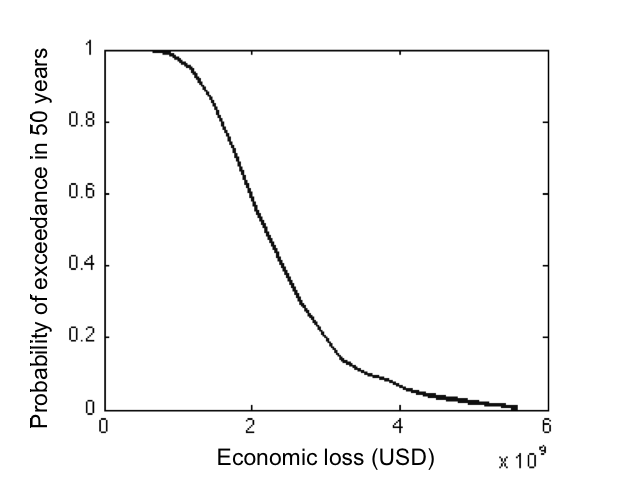
\includegraphics[width=7.5cm,height=6cm]{./Figures/Part_Risk/LossCurveIstanbul.eps} 
\caption{Aggregated loss exceedance curve for RC buildings.}
\label{fig:LossCurve}
\end{figure} 
 \begin{figure}[ht]
\centering
\includegraphics[width=12cm,height=9cm]{./Figures/Part_Risk/LossesProbIstanbul.eps}
\caption{Loss map for a probability of exceedance of 10\% in 50 years.}
\label{fig:ProbLosses}
\end{figure} 
